%%%%%%%%%%%%%%%%%%%%%%%%%%%%%%%%%%
\section{Il ruolo dell'esperimento ALICE}\label{ch:objectives_alice}
Come già anticipato, ALICE lavora su molti punti della ricerca nel campo della fisica delle particelle.
Coinvolgendo collisioni tra particelle pesanti, ALICE gioca un ruolo fondamentale nel rispondere al quesito dell'origine dell'universo.

\subsection{Studio della formazione nucleare}
Il principale obiettivo di ALICE è quello di studiare lo stato del plasma di quark e gluoni, il quale è ritenuto essere stato lo stato della materia negli istanti iniziali dell'universo, e in particolare la transizione da questa fase alla materia ordinaria, processo chiamato adronizzazione.
Infatti ALICE, tramite LHC e le collisioni di ioni pesanti, riesce a riprodurre e analizzare questo stato della materia, caratterizzato da temperature e pressioni estreme.
Tuttavia è importante menzionare che questo stato della materia ha vita breve, dell'ordine di $\sim10^{-23}$ s (come vedremo successivamente), e si misurano solamente i prodotti di decadimento, che consistono di particelle ordinarie come protoni, neutroni e nuclei leggeri, con le corrispettive antiparticelle.
Quindi ALICE si occupa anche dei meccanismi di formazione di nuclei che non sono ancora del tutto compresi; studiare la produzione dei (anti)nuclei leggeri potrebbe fornire informazioni su questi meccanismi e permettere di testare i modelli teorici che sono stati sviluppati per descriverli.

Più dettagli saranno forniti nel prossimo capitolo.

\subsection{Materia oscura}
Si studiano gli (anti)nuclei anche per un altro scopo, ossia la ricerca di materia oscura.
Si considera la materia oscura come la componente attrattiva dominante della gravità, ma, non potendola osservare direttamente, possiamo conoscere solamente alcune proprietà di essa, attraverso misure delle velocità di rotazione delle galassie, dispersione di velocità delle galassie ellittiche, lenti gravitazionali o comunque tramite osservazioni astronomiche.
Una eventuale scoperta della materia oscura porterebbe senz'altro a una rivoluzione senza precedenti nella fisica moderna.

Ad oggi abbiamo diversi modelli per caratterizzare la natura della materia oscura, in seguito ne elenchiamo alcuni: l'ipotesi barionica della materia oscura, per cui si ipotizza la composizione barionica della materia oscura; i modelli non barionici, come il modello degli assioni, ipotetiche particelle molto leggere e caratterizzate da elevate velocità, oppure il modello dei neutrini; infine, il più promettente, il modello dei WIMP.
Quest'ultimo modello, introdotto da Steigman e Turner \cite{STEIGMAN1985375_wimp}, ipotizza l'esistenza delle particelle massive debolmente interagenti, in acronimo WIMP (\emph{Weakly Interacting Massive Particle}). 
L'abbondanza di materia oscura può essere spiegata da questo modello, in particolare dal meccanismo di \emph{freeze-out} termico, nella quale il sistema, passando dal QGP, si espande così velocemente che la velocità dell'espansione dell'universo supera la velocità di interazione delle particelle.
Perciò si possono considerare i WIMP come i relitti termici dell'universo. 
Sebbene non siano stati ancora osservati sperimentalmente, neanche indirettamente, si predice che i WIMP annichilino e decadino in (anti)materia ordinaria (per esempio antiprotoni e antineutroni), i quali possono interagire formando stati legati, ossia antinuclei leggeri.
Questi possono invece costituire un segnale rilevabile, con energia cinetica di 0.1-1 GeV alla produzione, senza problemi di eventuali fondi cosmici, dal momento in cui alcuni dei modelli di WIMP predicono un flusso massiccio di antinuclei leggeri con ordini di grandezza in più rispetto a quello del fondo, come per esempio si può vedere in \autoref{fig:he3} per il nucleo di $^3\overline{\text{He}}$.
\begin{figure}[htb]
    \centering
    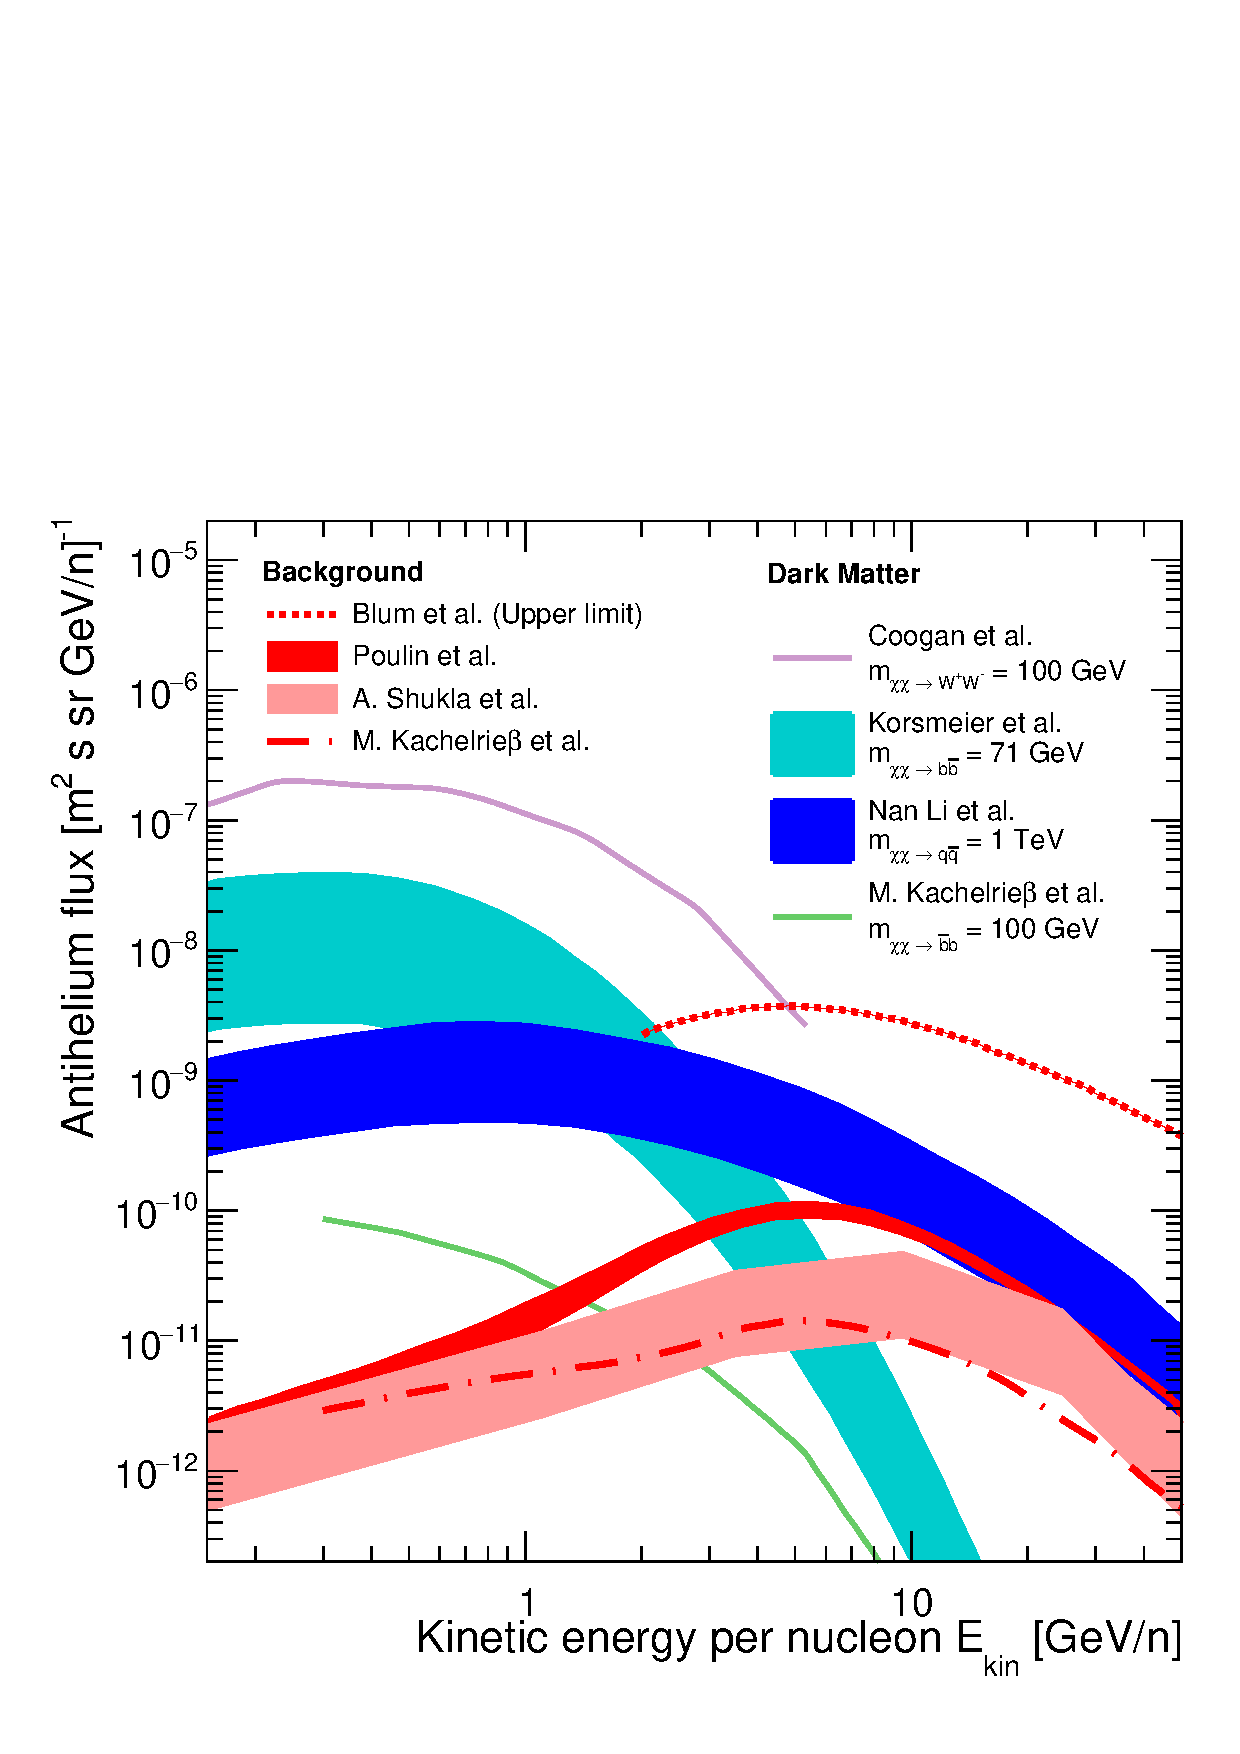
\includegraphics[width=0.6\textwidth]{image/1-alice/He3.pdf}
    \captionwithsource{Il flusso di $^3\overline{\text{He}}$ (in azzurro) in funzione dell'energia cinetica secondo più modelli di WIMP provenienti dalla letteratura scientifica, in confronto con il fondo cosmico (in rosso).}{\cite{Doetinchem_2020}.}
    \label{fig:he3}
\end{figure}

\subsection{La ricerca dei nuclei}
Per riuscire a studiare le proprietà degli (anti)nuclei è necessario come prima cosa riuscire a misurarli.
Tuttavia si noti che il numero di nuclei che viene prodotto in collisioni adroniche è molto ridotto, per cui un esperimento effettuato con un valore insufficiente dell'energia del centro di massa $\sqrt s$ comporta una percentuale molto bassa di (anti)nuclei prodotti.

Per quantificare questo numero, si considera che la formazione di un antinucleone è corrisposta necessariamente alla formazione di un nucleone, per conservazione del numero barionico.
Tenendo in considerazione ciò allora l'energia $\sqrt s$ dovrebbe assumere un valore molto più alto inizialmente.
% Per esempio per aggiungere il deuterone nel sistema è necessario l'aggiunta di 17 GeV in $\sqrt s$ \cite{2011STAREeuteronEormationEnergy}.
In generale nella letteratura si assume che venga prodotto un nucleo in ogni circa 1000 nucleoni prodotti, per nucleone del nucleo. 
Inoltre è necessario ricordare che in un evento di collisione il numero barionico deve essere conservato, per cui se l'energia iniziale è sufficientemente bassa, si vedrà uno sbilanciamento in numero, in particolare si avrà che il numero di antinuclei che vengono prodotti è più basso rispetto al numero di nuclei.
Per esempio, esperimenti condotti all'acceleratore \emph{Intersecting Storage Rings} (ISR) del CERN negli anni Settanta con collisioni pp ad energie del centro di massa di $\sqrt s \sim 50$ GeV hanno misurato un rapporto $D/\bar D$ di circa $4$ \cite{Gibson_Duane_Newman_Ogren_Henning_Jarlskog_Little_Sanford_Wu_B&Oslash;ggild_etal._2008}.

Per ovviare a questo problema è sufficiente aumentare il valore di $\sqrt s$.
Al LHC, l'energia è sufficientemente alta per poter portare il valore del rapporto di nucleo$/$antinucleo vicino a 1.
Per vedere questo, indicando con $D$ e $\bar D$ i deuteroni e gli antideuteroni rispettivamente, in \autoref{fig:ratio_of_matter/antimatter} riportiamo il grafico della frazione di $\bar p/p$ e di $\bar D/D$, dove si può osservare un avvicinamento al valore unitario con l'aumentare dell'energia.
\begin{figure}[htb]
    \centering
    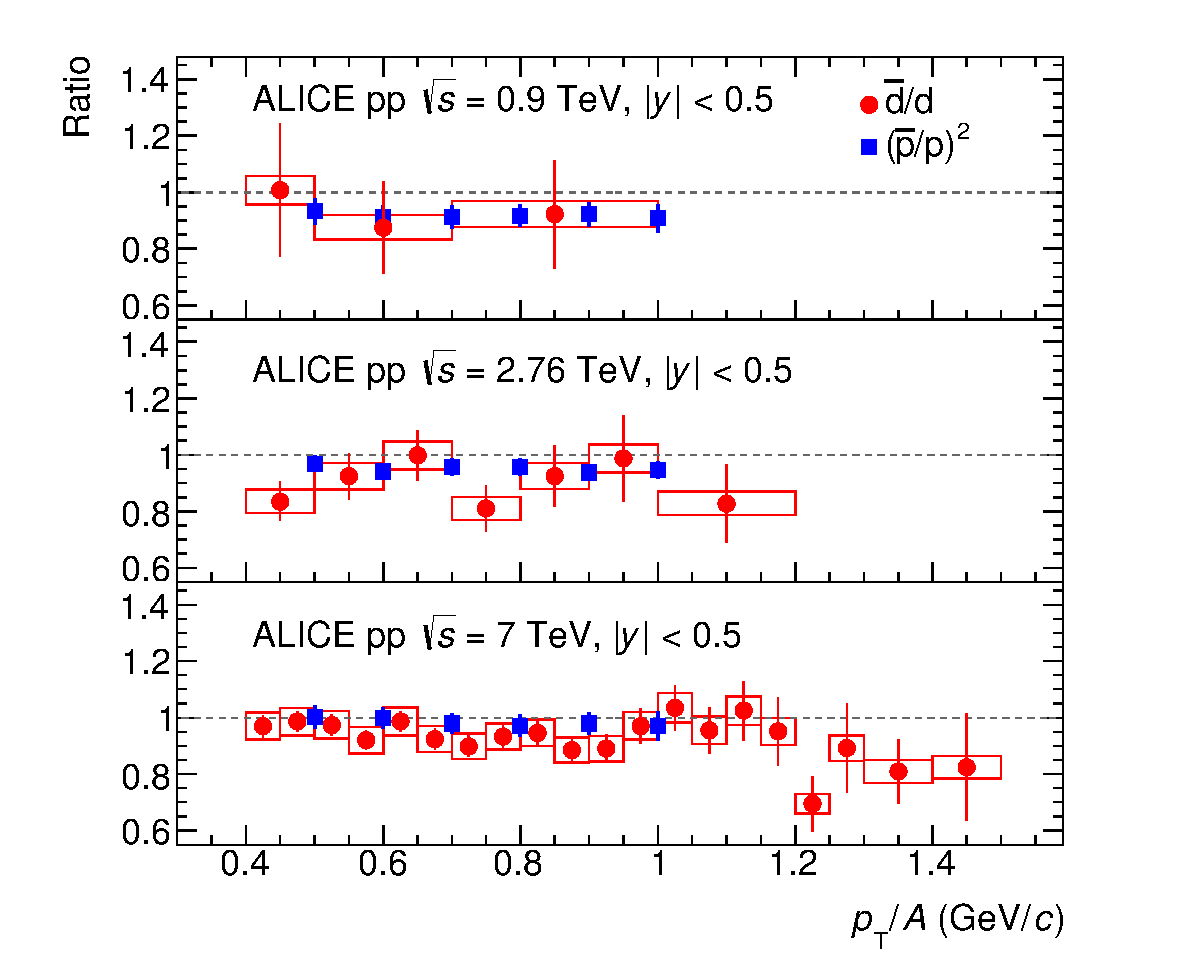
\includegraphics[width=0.7\textwidth]{image/1-alice/DbarDRatio.pdf}
    \captionwithsource{Andamento del rapporto di $\bar D/D$ (qui indicato con $\bar d/d)$ in funzione di $p_t$ per nucleone sovrapposta al rapporto quadro di $\bar p/p$, ai tre valori di energia indicati.}{\cite{Acharya_2018}.}
    \label{fig:ratio_of_matter/antimatter}
\end{figure}
